%---------------------------------------%
\subsection*{Question 4}
%2001 Question 4

\begin{itemize}
\item[(a)] A function $f$ is represented by the arrow diagram shown below.
\begin{center}
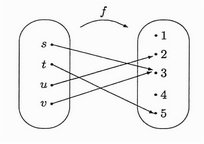
\includegraphics[scale=0.75]{HibCollArrow.jpg}
\end{center}

\begin{itemize}
\item[(i)] Give the domain, co-domain and range of $f$. [3 Marks]
\item[(ii)] Say why $f$ does not have the one-to-one property and why it does not
have the onto property, giving a specific counter-example in each case. [2 Marks]
\end{itemize}
\item[(b)]
\begin{itemize}
\item[(i)] State the conditions to be satisfied by a function $f : X \rightarrow Y$ for it to have
an inverse function $f^{-1} : Y \rightarrow X$. [3 Marks]
\item[(ii)] Define $f^{-1}$ when $X = \{1,2,3,4\}$, $Y = \{a,b,c,d\}$, and $f$ is given by the
table below. [2 Marks] \\
\begin{center}
\begin{tabular}{|c|cccc|}
  \hline
  % after \\: \hline or \cline{col1-col2} \cline{col3-col4} ...
  x & 1 & 2 & 3 & 4 \\ \hline
  f(x) & b & c & d & a \\
  \hline
\end{tabular}
\end{center}
\end{itemize}
\end{itemize}

